
Da  der Rohrofen bereits vorliegt und nicht ausgesucht werden muss, stellt sich eher die Farge wie sich das Material im Temperaturfeld verhält und wie sich das auf die Faserdicke auswirkt. Das Vorliegende

\begin{wrapfigure}{l}{0.5\textwidth}
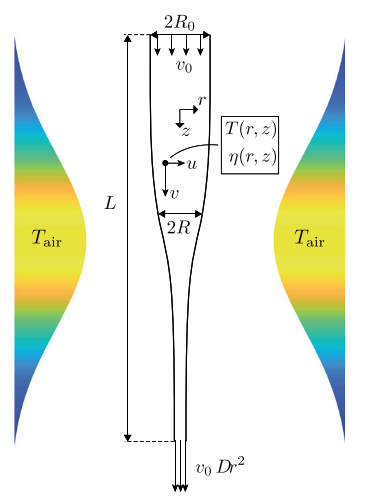
\includegraphics[width=0.9\linewidth]{Abbildungen/temp_field_clear.png} 
\caption{Temperaturfeld im Rohrofen
\cite{Page.2019} \vspace{1mm}}
\label{fig:thermal_field}
\end{wrapfigure}
 Berechnungsmodell bezieht sich ausschließlich auf Systeme welche vom verhalten durch ihr Mantelmaterial bestimmt sind. Es beschreibt das System im 2-Dimensionalen Raum, durch die Ausdehnenung $R(z)$ entlang der Hauptachse sowie durch ein Beschleunigungsfeld $u(r,z)$ in radialer- und $v(r,z)$ in axialer Richtung. Weiternen Einfluss nehmen das Temperaturfeld $T(r,z)$ sowie die Scherviskosität $\eta(r,z)$\cite{Page.2019}. Vorraussetzung für die Anwendbarkeit ist das vorhandensein einer dünnen Faser.
 \begin{equation}
     \alpha^2 = (\frac{R_0}{L})^2 \ll 1 \hspace{5mm}\cite{Page.2019} Gl.(1)
     \label{eq:fiber_thick}
 \end{equation}
Für den Fall des vorhandenen Ofens ergibts sich miitels Gleichung \ref{eq:fiber_thick} 
\begin{equation*}
    (\frac{R_{0max}}{L})^2 = (\frac{45mm}{500mm})^2 =8,1*10^{-3}
\end{equation*}
ein Wert der deutlich unter eins liegt und die Bedingung somit erfüllt.

\vspace{20mm}
 
Die größte unbekannte Unbekannte im Entwicklungsprozess ist das Fließverhalten des Halbzeugs. Da die bimorphe Faser aus mehren Materialien mit verschiedenen thermodynamischen Eigenschaften besteht, ist das Verhalten bei der Erwärmung schwer abzuschätzen. Da zum Zeitpunkt der Auslegung die Materialkombination nicht vorliegt, wird mit einer groben Näherung über die Kontinuitätsgleichung (Gl. (\ref{eq:kntinuitätsgleichubng})) gearbeitet.
\begin{equation}\label{eq:kntinuitätsgleichubng}
    v_1*A_1 = v_2*A_2
\end{equation}
Da die möglichen Durchmesser des Halbzeuga ($d_1 = [10, 45]mm$) sowie die  der  Faser ($ d_2 = [50*10^{-3}, 2]mm$) aus den Anforderungen hervorgehen, kann mit den Messwerten aus den Vorversuchen eine Abschätzung des Verhaltens getroffen werden.
\begin{equation}\label{eq:speed_v2}
    v_1 = v_2 * \frac{d_2^2}{d_1^2}
\end{equation}
Für die gemessene Materialkombination \acs{pla}/\acs{pla} ergibt sich mittels Gleichung \ref{eq:speed_v2} die folgende Fördergeschwindigkeit.
\begin{equation*}
    v_1 = 72\frac{mm}{s}*\frac{(358 * 1^{-3}mm)^2}{(18,5mm)^2} \approx 26,96 \frac{\mu m}{s}
\end{equation*}
Da davon Auszugehen ist das sich nicht alle Materialien gleich verhalten oder sich die Form der Probenkörper ändert wird der benötigte Geschwindigkeitsbereich um die Werte aus dem Versuch hervorgegangenen sind approximiert. 

\begin{figure}[!h]
     \centering
     \begin{subfigure}[]{0.4\textwidth}
         \centering
         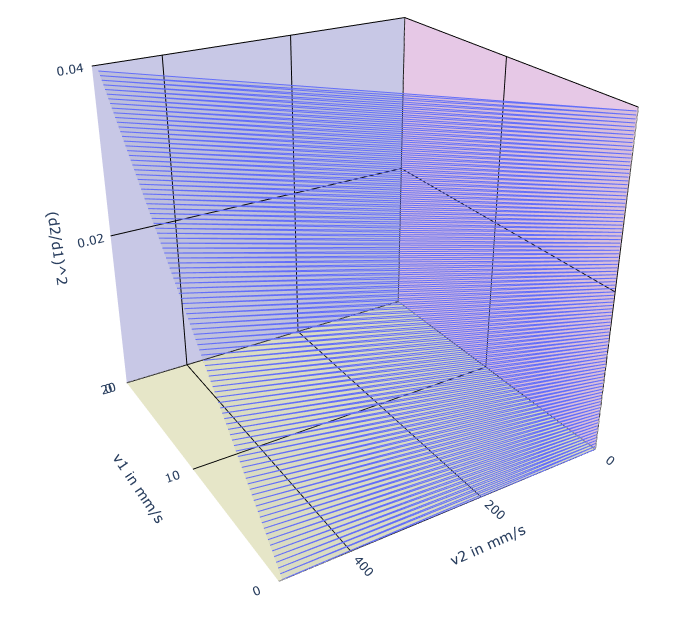
\includegraphics[width=\textwidth]{Abbildungen/v1_v2_d_wirframe_2 (2).png}
         
         \label{fig:abzug_speed}
     \end{subfigure}
     \hspace{0mm}
     \begin{subfigure}[]{0.2\textwidth}
         \begin{align*}
             v_{1min} = &  \ 1 \frac{mm}{s} * (\frac{200*10^{-3}mm}{45mm})^2 \approx 0,0198 \frac{\mu m}{s}\\      
             v_{1max} = &  \ 500  \frac{mm}{s} * (\frac{2mm}{10mm})^2 \approx 20 \frac{mm}{s}
         \end{align*}
         
         \label{fig:abzug_min_max}
     \end{subfigure}
     \caption{Abzugsgeschwindigkeiten}
      \label{fig:abzugsgeschwindigkeit}
\end{figure}

Die Entscheidung 500 $\frac{mm}{s}$ (Abbildung \ref{fig:abzugsgeschwindigkeit}) als maximale Abzugsgeschwindigkeit anzunehmen ist daraus begründet, das die im Versuch entstandene Faser bereits sehr nah an der unteren Dickengrenze liegt und das die Viskosität des Materials im Versuch sehr niedrig war. Deshalb gehe ich davon aus das ein Sicherheitsfaktor von circa 7 in der Abzugsgeschwindigkeit für viele mögliche Materialkombinationen ausreichend ist. 
So ergeben sich am ende zwei Geschwindigkeitsbereiche, einer für den Abzug und einer für die Materialfördereinheit. Dabei sit $v_1$ die Zuführgeschwindigkeit und $v_2$ die Abzugsgeschwindigkeit.
\begin{equation*}
    v_1 = [0,198\frac{\mu m}{s}; 20 \frac{mm}{s}] \hspace{20mm} v_2 = [1\frac{mm}{s};500\frac{mm}{s}]
\end{equation*}
         

 \newpage